\documentclass[conference]{IEEEtran}
% If the IEEEtran.cls has not been installed into the LaTeX system files,
% manually specify the path to it.  e.g.
% \documentclass[conference]{./IEEEtran}

% Add and required packages here
\usepackage{graphicx,times,amsmath,fontenc,multirow,url,caption}
%\usepackage[top = 25mm, left = 19mm, right = 19mm, bottom = 19mm]{geometry}

% To create the author's affliation portion using \thanks
\IEEEoverridecommandlockouts

%\textwidth 178mm
%\textheight 239mm
%\oddsidemargin -7mm
%\evensidemargin -7mm
%\topmargin -6mm
%\columnsep 5mm
\begin{document}

% Paper title: keep the \ \\ \LARGE\bf in it to leave enough margin.
\title{\ \\ \LARGE\bf Measuring Interestingness of Continuous Game Problems }

\author{Samuel A. Roberts, Simon M. Lucas}

% Uncomment out the following line for invited papers
%\specialpapernotice{(Invited Paper)}

% Make the title area
\maketitle

\begin{abstract}

This paper investigates the relationship between the difficulty and the interestingness of individual problem candidates from within a class of related problems, using {\itshape Lunar Lander} as a case study. In this class of problems, a 2D spaceship must be controlled by a simple set of macro-actions, including both linear and angular impulses, such that it fulfils a set of weighted criteria relating to landing on a jagged landscape with flat landing pads. 
%These weighted criteria involve landing with a low velocity, landing as close to a landing pad as possible, conserving fuel expended during movement and landing in a proper orientiation. The individual problems themselves vary by their environmental parameters as well as the weights dictating how important these criteria are.
It is demonstrated that a very simple measure based on standard deviations of improvement can be used to guide evolution to develop interesting problems in this class of problems, which in turn can be solved using evolution strategies to get a high level of improvement based on initial random performance. We examine the impact of the measure used on the evolution of the problems, and also what aspects of this problem class affect the difficulty and interestingness the most. 

\end{abstract}

% No keywords

\section{Introduction}

This paper describes an investigation into how the difficulty of a problem relates to how interesting a problem is to solve, and how a problem can be determined and quantified as interesting. Building upon previous research and experience, the case study is a problem inspired by the arcade game of {\itshape Lunar Lander}, wherein a spaceship is piloted to land on a surface at a low velocity. The chosen approach to solving this problem consists of generating and optimising a set of actions, through evolution, to provide a spaceship trajectory which lands with minimal error. This error is determined by the fulfilment of certain sub-conditions. These sub-conditions, and their relation to the performance of the generated solutions, in turn affect the difficulty and interest of the problem, as do the features of the problem environment. As the elements of a problem are investigated, it becomes increasingly clear that the combination and weighting of elements of a suitability measure have a drastic impact on the difficulty of a problem and the effectiveness of the solutions.

\subsection{Motivation}

\subsubsection{Effect of Constraints on Difficulty of Problems}

It has been shown in the past that the constraints of a problem have a dramatic effect and impact on the difficulty and solvability of a problem \cite{kramer10}, and that trivial problems can be made far more difficult with the weight of additional constraints. One of the main inspirations for this study came from reusing techniques used in a similar environment in an environment closer to {\itshape Lunar Lander}, and finding that the general problem itself was much harder to solve than would have otherwise been expected. In carrying out this research, it is hoped that some explanation as to what makes realtime game problems like the focus of this paper so much more difficult and time-consuming to solve than similar problems. The focus is on, in particular, the conditions that drive this difficulty, and what about these conditions causes this spike in difficulty to occur.

\subsubsection{Quantifying Interestingness of Problems}

Investigating into what factors drive this difficulty is worthy in its own right, as the insights achieved here could easily be applied to other problems. Attempting to define and utilise a simple means for quantifying the interestingness of a specific problem, out of a class of related problems, can give insight as to whether such a method can be useful in other domains. If the interestingness of a problem can be easily quantified, then deriving a process to generate problems that are interesting becomes a simple matter of optimisation. This can then be achieved by any number of standard methods, such as evolution strategies. Previous work has examined the idea of interestingness or impressiveness in generating novel artefacts \cite{lehman12}, with the notion of interestingness relating to the hypothetical difficulty of reconstructing said artefacts from an initial blank slate. In this work, we examine a notion of interestingness based upon the difficulty of solving a problem given certain environmental parameters, as the focus is more on dynamic problems than the creation of interesting artefacts. 

\subsubsection{Examining Constraint Impact in a Game Context}

The work undertaken here relates to the concept of co-evolving separate populations that co-operate in their evolution to produce better results \cite{potter94}, an approach which has also been demonstrably useful in completely automated game design \cite{cook12}.
It more strongly relates to other investigations along similar lines of evolving the environment used to evolve solutions to an inner problem, such as procedural generators that generate procedural level generators \cite{kerssemakers12}. Through evolution of the environment, the impact on the evolved control sequences for video game entities can be clearly observed. It is also possible that what constitutes an interesting problem to solve in this context when attempting evolution may correlate to engineering an interesting problem for players to solve, adding to the fun \cite{koster04} \cite{pedersen10} of a given game for the player. 

\subsubsection{Automated Game Design}

As has been demonstrated in the past \cite{brown10}, it is entirely possible that an automated game designer or design tool could be implemented and driven by some measure of a game's interestingness. By dynamically analysing whether a particular set of parameters is more interesting or not, it becomes easier to automate the process of refining elements of a game's design or to construct them from scratch. This measure could either similar to the one presented within this paper, based upon the progress made by attempting to find solutions to the game, or by some other definition of interestingness. 

\subsection{Prior Research}

The choice of {\itshape Lunar Lander} as a test case for this research is inspired by previous research \cite{roberts12} on procedural generation of spaceships in a game with {\itshape Asteroids} style physics. The primary physics of a ship with complete freedom of rotation and the ability to thrust only in the current heading of the ship are common across both games. However, {\itshape Lunar Lander} has the addition of gravity as a constant force and a landscape that serves both as the primary goal and the primary obstacle.
A method called Covariance Matrix Adaptation Evolutionary Strategy (CMA-ES) \cite{hansen06} is used to evolve a vector representing a set of macro actions in the inner problem defined by the parameters of a given problem candidate, and to evolve a vector representing parameters of the problem environment in the outer problem of designing an interesting problem.

\section{Methodology}

\subsection{Software Implementation}

For the evolutionary algorithm used in both cases requiring an evolutionary algorithm, we used a freely available Java version of
CMA-ES\footnote{\url{http://www.lri.fr/~hansen/cmaes_inmatlab.html}}, without significant modification. 

\subsection{Environment and Physics}

Before much can be said about defining the parameters of the environment of the problem, which constitutes the outer problem, the details of the inner {\itshape Lunar Lander} inspired problem must first be made clear.

The basic environment consists mostly of a two-dimensional space and a landscape. Vehicles that move out of horizontal bounds are not moved to the opposite horizontal edge of the space, as in some {\itshape Lunar Lander} implementations, for the simple reason of allowing for a more linear measure of ship proximities further ahead. The co-ordinate space used within this environment defines the origin to be at the top-left of the world, much as is defined for co-ordinate systems relating to display systems. 

\begin{figure}[hbtp]
\centering
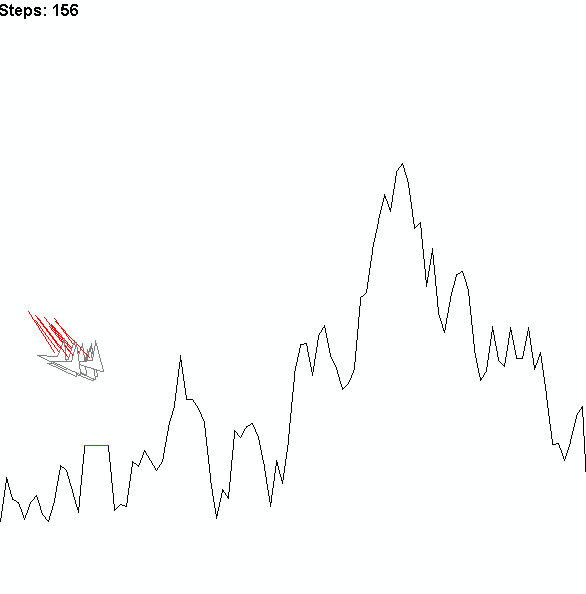
\includegraphics[scale=0.53]{img/lunarlandscape}
\caption{A view of ships within this environment.}
\label{fig:lunarlandscape}
\end{figure}

The landscape is generated through a fixed random seed that is determined during experimental set-up. It is generated as a series of line segments based on generated vertices, each equally distributed horizontally and distributed semi-randomly within a specific range of the game world vertically. The landscape is represented as a vector; as the points are horizontally spaced, the horizontal position of each vertex of the landscape is a function of the vector index. The vertical component of the first point is defined to be a fraction of the world height, $c$. Each subsequent point has a vertical component based on a random number taken from a scaled normal distribution, added to the vertical component of the previous vertex's vertical component. For a number of points, $n$, and a world width $w$ and height $h$, the initial point $\boldsymbol {p}^{0}$ is defined as:

\begin{equation} 
\boldsymbol {p}_{x}^{0} = 0
\end{equation}
\begin{equation} 
\boldsymbol {p}_{y}^{0} = c
\end{equation} 

The arbitrary point $\boldsymbol {p}_{i}$, where $i \neq 0$, and $\sigma$ is the scale factor, is defined as:

\begin{equation}
\boldsymbol {p}_{x}^{i} = \frac{iw}{n} 
\end{equation}
\begin{equation}
\boldsymbol {p}_{y}^{i} = \boldsymbol {p}_{y}^{i-1} + \sigma\mathcal{N}(0,1)
\end{equation}

This process is repeated until the entire vector of $y$ values is populated, forming the landscape. Once this has been created, the landing pads are generated through a similar procedure, but are instead represented as pairs of values; the initial index or scaled $x$ component of the point where the landing point begins, and the length in points of the landing pad. These initial indices are selected randomly, with the lengths predefined during the experiment setup, and are created simply by setting the vertical component of all landing pad points to be equal to the initial landing pad point. In the event a landing pad would begin at the right of the landscape and be too long to fit on the landscape, it wraps around to the other side of the landscape.

In order to allow the collision of vehicles with the landscape, it is necessary to be able to determine whether a point in the two dimensional space falls within the lunar landscape. Firstly, it is determined whether or not the vehicle is currently present within the horizontal range of the landscape, which is a simple boundary check on the horizontal component of the vehicle's position. After confirming the vehicle is within the horizontal boundaries of the landscape, all that is required is to determine if the vertical component of the point is equal to or greater than the vertical component of the point projected to the landscape.

\begin{figure}[hbtp]
\centering
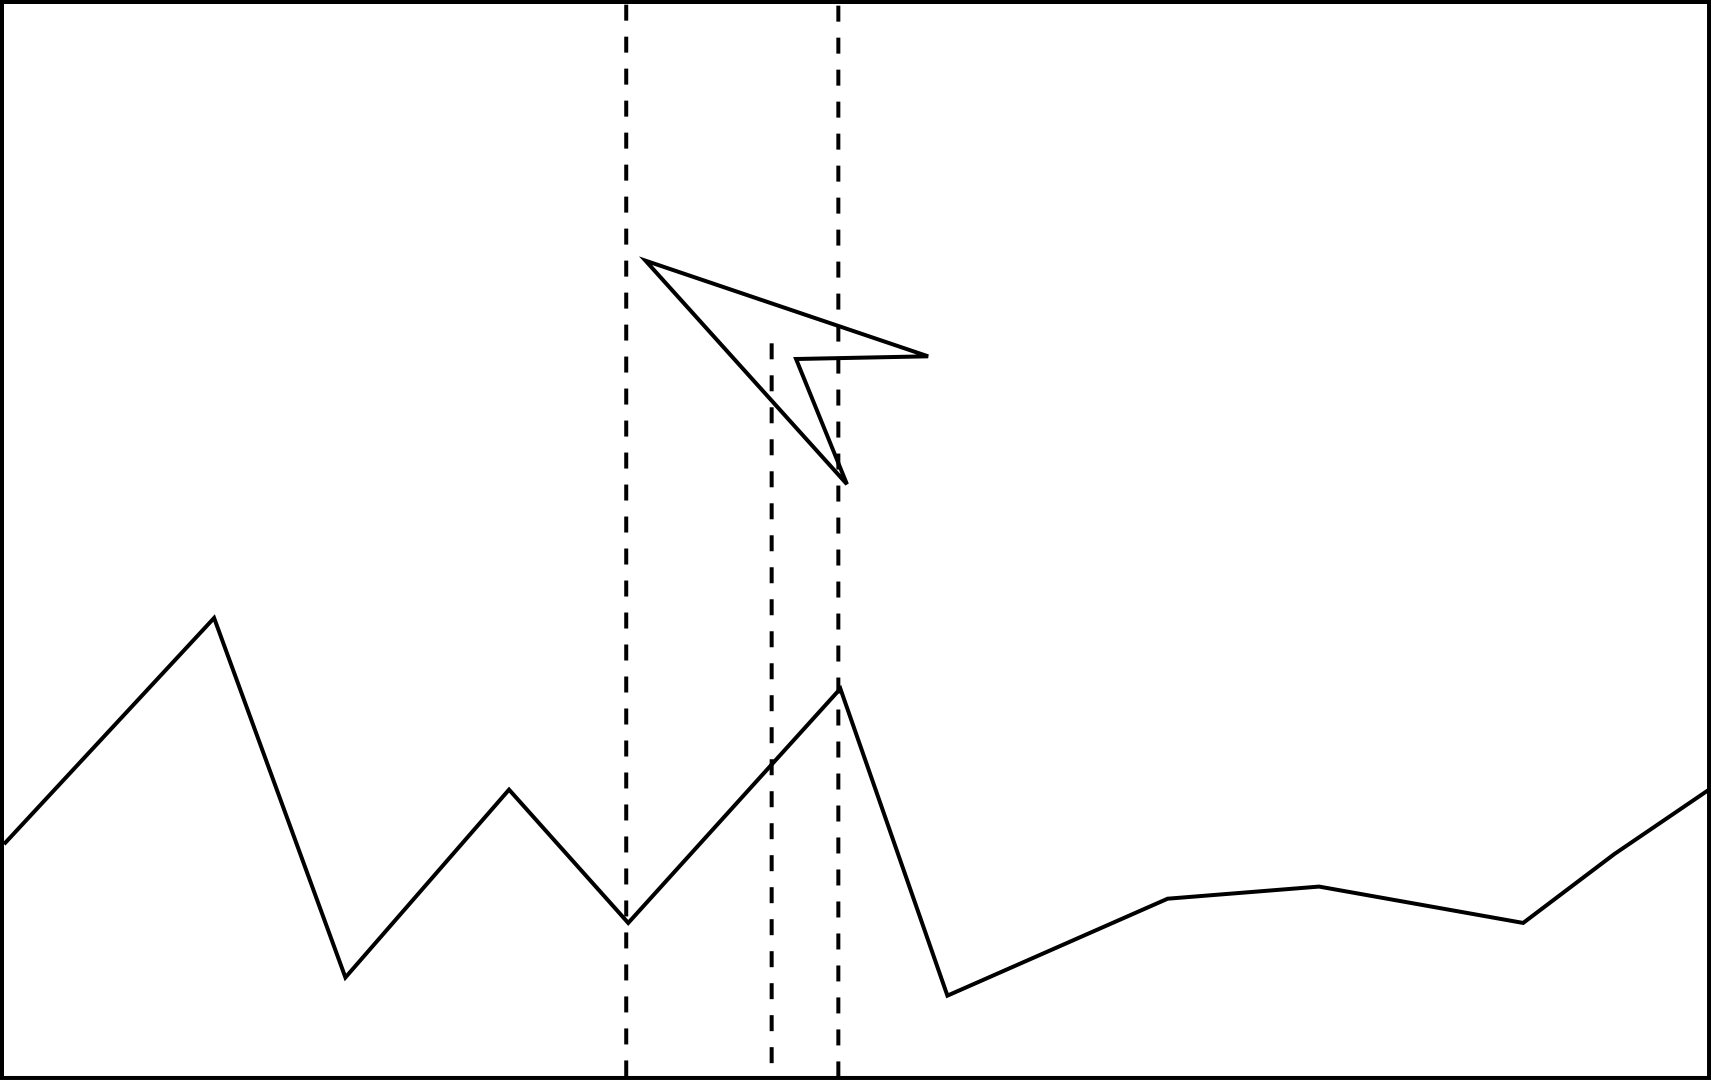
\includegraphics[scale=0.5]{img/landscapepoint}
\caption{The point closest to the spaceship on the landscape lies in between two of the defined vertices of the landscape, and requires interpolation to calculate the y co-ordinate from the x co-ordinate of the ship.}
\label{fig:graph_landscapepoint}
\end{figure}

This can be achieved by determining the closest leftmost discrete point of the landscape to the point being queried, and interpolating the $y$ component of the closest landscape point from there. For a given query point of $\boldsymbol {q}$, the equivalent index $i$ in the vector of points of length $n$ can be determined simply through $floor(\frac{\boldsymbol {q}_{x}}{n})$. The interpolation value, $v$, is equal to $\frac{\boldsymbol {q}_{x}}{n} - i$. From there, the landscape point $\boldsymbol {l}$ that corresponds is:

\begin{equation}
\boldsymbol {l}_{x} = \boldsymbol {q}_{x}
\end{equation}
\begin{equation}
\boldsymbol {l}_{y} = \boldsymbol {l}_{y}^{i} + v\boldsymbol {l}_{y}^{(i+1)\bmod{n}}
\end{equation}

In addition to the physical properties of the landscape, the environment can also act upon entities within it with a gravity force and a velocity loss factor, both of which are defined before the experiment begins. Gravity is simply an addition to the vertical component of any entity capable of movement each step, which includes all vehicles, while the loss factor is any value $n$ where $0 \le n \leq 1$. Both the linear velocity and angular velocity of any entity in the environment is multiplied by this loss factor, allowing for modelling resistance of the environment, or no resistance at all. 

\subsection{The Vehicle}
Within this environment, a vehicle has a few fixed physical properties. It is modelled as a circular mass, possessing a position in the two-dimensional space of the simulation, $\boldsymbol {s}$, a rotation, $\theta$, a radius, $r$, a mass, $m$, a centre of mass, $\boldsymbol {R}$, and a moment of inertia, $I$. In addition, a vehicle will also possess a linear velocity, $\boldsymbol {v}$, and an angular velocity, $\omega$. At the beginning of a simulation, every single one of these values will be set to a constant default, allowing for entirely deterministic outcomes given the same macro actions.

The vehicle is capable of both turning through angular impulses and moving through linear impulses. These linear and angular impulses are provided by the macro actions that govern the behaviour of the ship during the simulation, and will be discussed in more detail later. All linear forces applied to the ship are applied as a single value, causing a linear acceleration based on the current heading of the ship. This thrust value, $a_{T}$, is restricted according to two rules. Firstly, linear force applied to the ship cannot be negative, and a thrust value below zero is corrected to zero. Secondly, the thrust value cannot exceed the thrust limit, $a_{max}$, as defined in the experiment. Any thrust value that would exceed this value is set instead to this value. The thrust value therefore always meets the condition of $0 \leq a_{T} \leq a_{max}$.

The vehicle collides with the landscape based upon the lowest point of its bounding circle colliding with the highest point, $\boldsymbol {l}$ of the landscape on the same horizontal axis. Collision occurs if the following condition is true:

\begin{equation}
\boldsymbol {s}_{y} + r \geq \boldsymbol {l}_{y}
\end{equation}

If this condition is true, the ship has collided with the landscape, and has either landed or crashed based on the survivable velocity threshold determined for the experiment. A simulation where the ship has landed or crashed is immediately halted and scored.

Each vehicle is supplied with an initial amount of fuel, which can vary based on experimental set-up. This fuel is consumed each and every step of the simulation based upon the amount of {\itshape forward} thrust applied to the vehicle. Rotational impulses do not reduce fuel, as in {\itshape Lunar Lander}. For a given thrust amount, the amount of fuel consumed per step is exactly equal to the thrust, factoring in the thrust limit. An amount of thrust that has already been capped by the thrust limit will consume an amount of fuel equal to the thrust cap.

\subsection{Vehicle Control and Solutions}

The solutions provided to the problem consist of a vector representative of set of macro actions. In this context, a macro action is an action that is repeated without interruption for a number of timesteps until its completion. The controller for the vehicle simply uses the set of macro actions provided through evolution to control the vehicle. The success of the vehicle in landing is entirely dependent on the suitability of the evolved set of macro actions as a means of controlling the vehicle.

A macro action is composed of three values. These values are the linear impulse applied to the ship each frame the action is active, the rotational impulse applied, and the number of timesteps the macro action is active for. Once the macro action has been executed for a number of frames either equal or greater to the number of timesteps it should be active for, the controller will use the next macro action in the set of macro actions provided to it through evolutionary means.

A set of macro actions is represented as a vector. Once the last set of three values is executed, the controller will wrap around to the beginning of the vector and continuing executing the macro actions from the first defined macro action. This will repeat until the vehicle has landed or the simulation has stopped after reaching the maximum allowed number of timesteps.

\begin{figure}[hbtp]
\centering
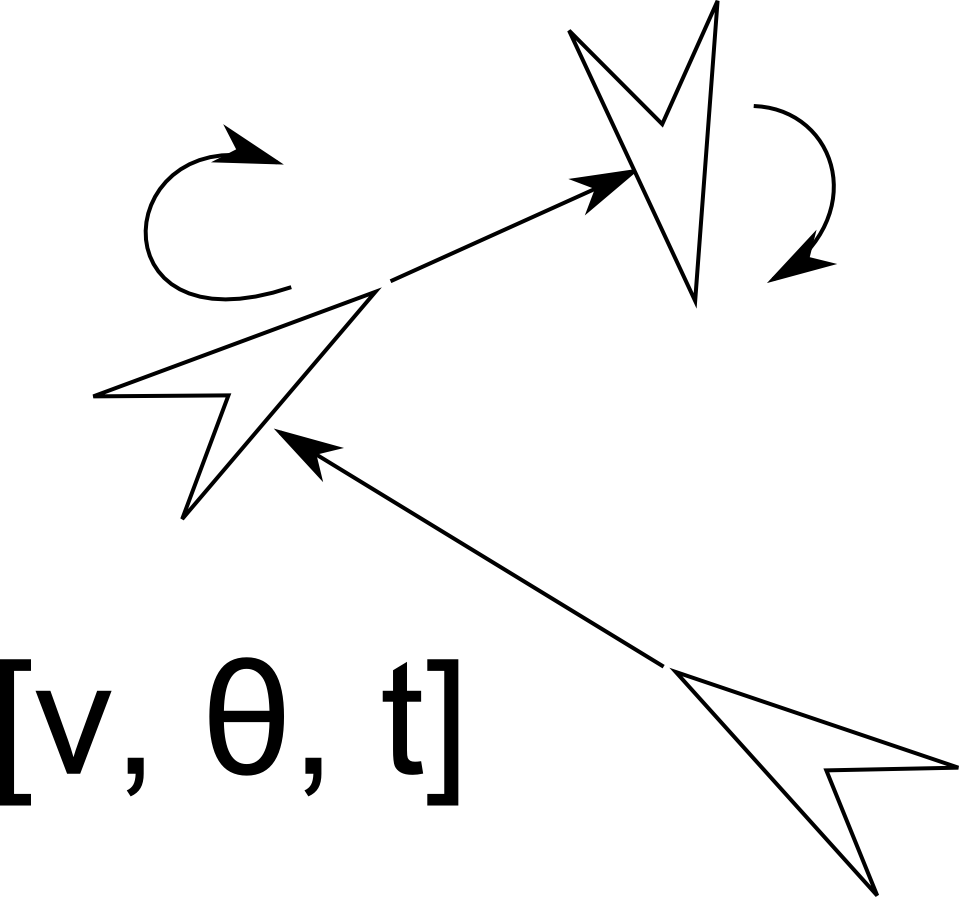
\includegraphics[scale=0.5]{img/macroaction}
\caption{Each set of three doubles determines the linear thrust, the angular impulse and the amount of steps to repeat the action for. Upon finishing the action, the next action is used. When the last action is used, the first action is used afterwards and the process repeats.}
\label{fig:graph_macroaction}
\end{figure}

These vectors of macro actions constitute the solutions that are evolved within the constraints of the outer problem, which in turn has its parameters set through evolution. There are, in effect, two evolutionary processes at work during any given experiment, with one evolutionary process guiding the parameters of the problem and a nested inner evolutionary process generating solutions for the problem given those parameters.

\subsection{Solution Suitability Measure}

The suitability measure used has a small but significant set of sub-conditions with associated weights. These measures measure the error of the current situation and a hypothetical perfect solution, and as such produce values intended to be minimised as opposed to maximised.

\subsubsection{Velocity}
One of these sub-conditions measures the velocity of the vehicle upon collision with the land. The priority for this sub-condition is to minimise the velocity upon impact. The magnitude of the velocity, $|\boldsymbol {v}|$, penalising all velocity above the survivable velocity threshold, $v_{t}$. Given the weighting $w_{v}$, the contribution, $c_{v}$ to the final score is

\begin{equation}
c_{v} = \max (0, w_{v}(|\boldsymbol {v}| - v_{t}))
\end{equation}

\subsubsection{Proximity}
Another sub-condition measures the proximity of the vehicle to the nearest landing pad to it upon landing. The priority for this sub-condition is to minimise the horizontal distance between the vehicle and the nearest landing pad. In the rare but possible event there exists no landing pad, the world origin of $<0, 0>$ is used as a substitute, effectively allowing for a default landing pad position if none is given. The distance to the nearest landing pad's centre is calculated as $\boldsymbol {l}^{p}$. Given the weighting $w_{d}$, the contribution, $c_{d}$ to the final score is

\begin{equation}
c_{d} = w_{d}|\boldsymbol {s}_{x} - \boldsymbol {l}_{x}^{p}|
\end{equation}

\subsubsection{Landing Angle}
This sub-condition measures how close the landing angle of the vehicle is to the ideal angle of being perfectly perpendicular to the flat landing pad, with a heading facing vertically upwards. To calculate this, a unit vector representative of the ideal landing heading, $\boldsymbol {h}$, is rotated by the ship's rotation $\theta$, to give the rotated heading vector $\boldsymbol {h}^{\theta}$. Given the weighting $w_{a}$, the contribution, $c_{a}$ to the final score is

\begin{equation}
c_{a} = w_{a}(\arccos(\boldsymbol {h} \cdot \boldsymbol {h}^{\theta}))
\end{equation}

\subsubsection{Fuel Consumption}
This last sub-condition measures the efficiency of the fuel usage in a simulation. The priority for this is on low fuel usage. It is simple to calculate given the fuel consumed, $f$, and the initial fuel amount, $f_{0}$. Given the weighting $w_{f}$, the contribution, $c_{f}$ to the final score is

\begin{equation}
c_{f} = w_{f}(f_{0} - f)
\end{equation}

\subsubsection{Total Effectiveness}
Given these component objectives, the final measure of the effectiveness of a solution, $f$, is

\begin{equation}
f = c_{v} + c_{d} + c_{a} + c_{f} 
\end{equation}

\subsubsection{Alternate Measure}

In the event that a solution does not result in a spaceship colliding with the landscape, an alternate measure is used. As the aim is to minimise the error, this value is enlarged to encourage any solutions that result in landings instead of aimless movement in the space above the landscape for the full length of allotted timesteps. As such, the effectiveness of a solution $f$, when the ship has failed to land, is defined based on the absolute distance of the y co-ordinate of the ship, $\boldsymbol {s}_{y}$, to the y co-ordinate of the landscape, $\boldsymbol {l}_{y}$, on the same vertical line of the ship. Hence, $f$ becomes

\begin{equation}
f = 100|\boldsymbol {s}_{y} - \boldsymbol {l}_{y}|
\end{equation}

By multiplying by this factor, even the worst results of landing with the landscape become an improvement to the case where spaceships do not even land. This encourages solutions which land and from there the course of evolution can shape the landings into better quality landings, if the problem constraints allow for it.

\subsection{Problem Representation}

Given the above measures all apply to the inner {\itshape Lunar Lander} inspired problem, the outer problem constitutes finding a set of environmental parameters that lead to an interesting evolutionary progress in solving the inner problem. These environmental parameters are represented as a vector of doubles that correspond to specific parameters, based on their ordering. These doubles are then transformed into values more appropriate for their corresponding parameters. There are thirteen parameters in total that vary and are adjusted in the course of evolution.  The parameters that are varied are those included in Table \ref{tab:params}, as well as the weightings on the four sub-conditions discussed earlier. The weightings for these conditions default to a value of $1$ for all sub-conditions, save for the fuel conservation sub-condition, which defaults to a value of $0$.

\subsection{Problem Interestingness Measure}

A candidate problem is evaluated through simple statistical analysis of the progress of evolution that takes place according to the parameters of said candidate problem. Firstly, in order to have a baseline to compare the progress of solving the problem to, an initial population of 1000 random individuals is generated and evaluated with the environmental parameters as specified for the problem candidate. From the fitness scores of these individuals, a mean fitness for this random population is calculated, $f_{\bar{u}}$, which approximates the general performance of unimproved solutions to the problem. Also calculated is the standard deviation of the population fitness, $\sigma$.

Given this baseline fitness measure, evolution is performed on a population of individuals in the standard manner, attempting to find as optimal a solution as can be found to the problem within a predetermined number of fitness measure evaluations, as specified in Table \ref{tab:const}. Upon completion, the best discovered fitness, $f_{b}$, is stored. The interestingness of the problem can be calculated with these values based on the number of standard deviations of improvement from the baseline performance fitness. This simple measure of the interestingness of a problem, $f_{p}$, is

\begin{equation}
f_{p} = \frac{f_{b} - f_{\bar{u}}}{\sigma}
\end{equation}

This measure is used as it is a simple and intuitive measure of the progress made in improving solutions to the problem. A higher number of standard deviations of improvement necessarily implies a higher level of improvement. If the numerical value of the standard deviations is low, this implies that the problem is incredibly difficult to solve through random generation, as opposed to through a guided process such as evolutionary search, and a high amount of improvement suggests that there is a high level of improvement that can be made with a more guided attempt to solve the problem, making it an interesting problem to investigate, as well as indicating that it is a problem wherein noteworthy progress can be made.

For each problem candidate, the final measure of the candidate's interestingness is averaged over three runs to prevent random chance producing misleading outlier results.

\begin{figure}[hbtp]
\centering
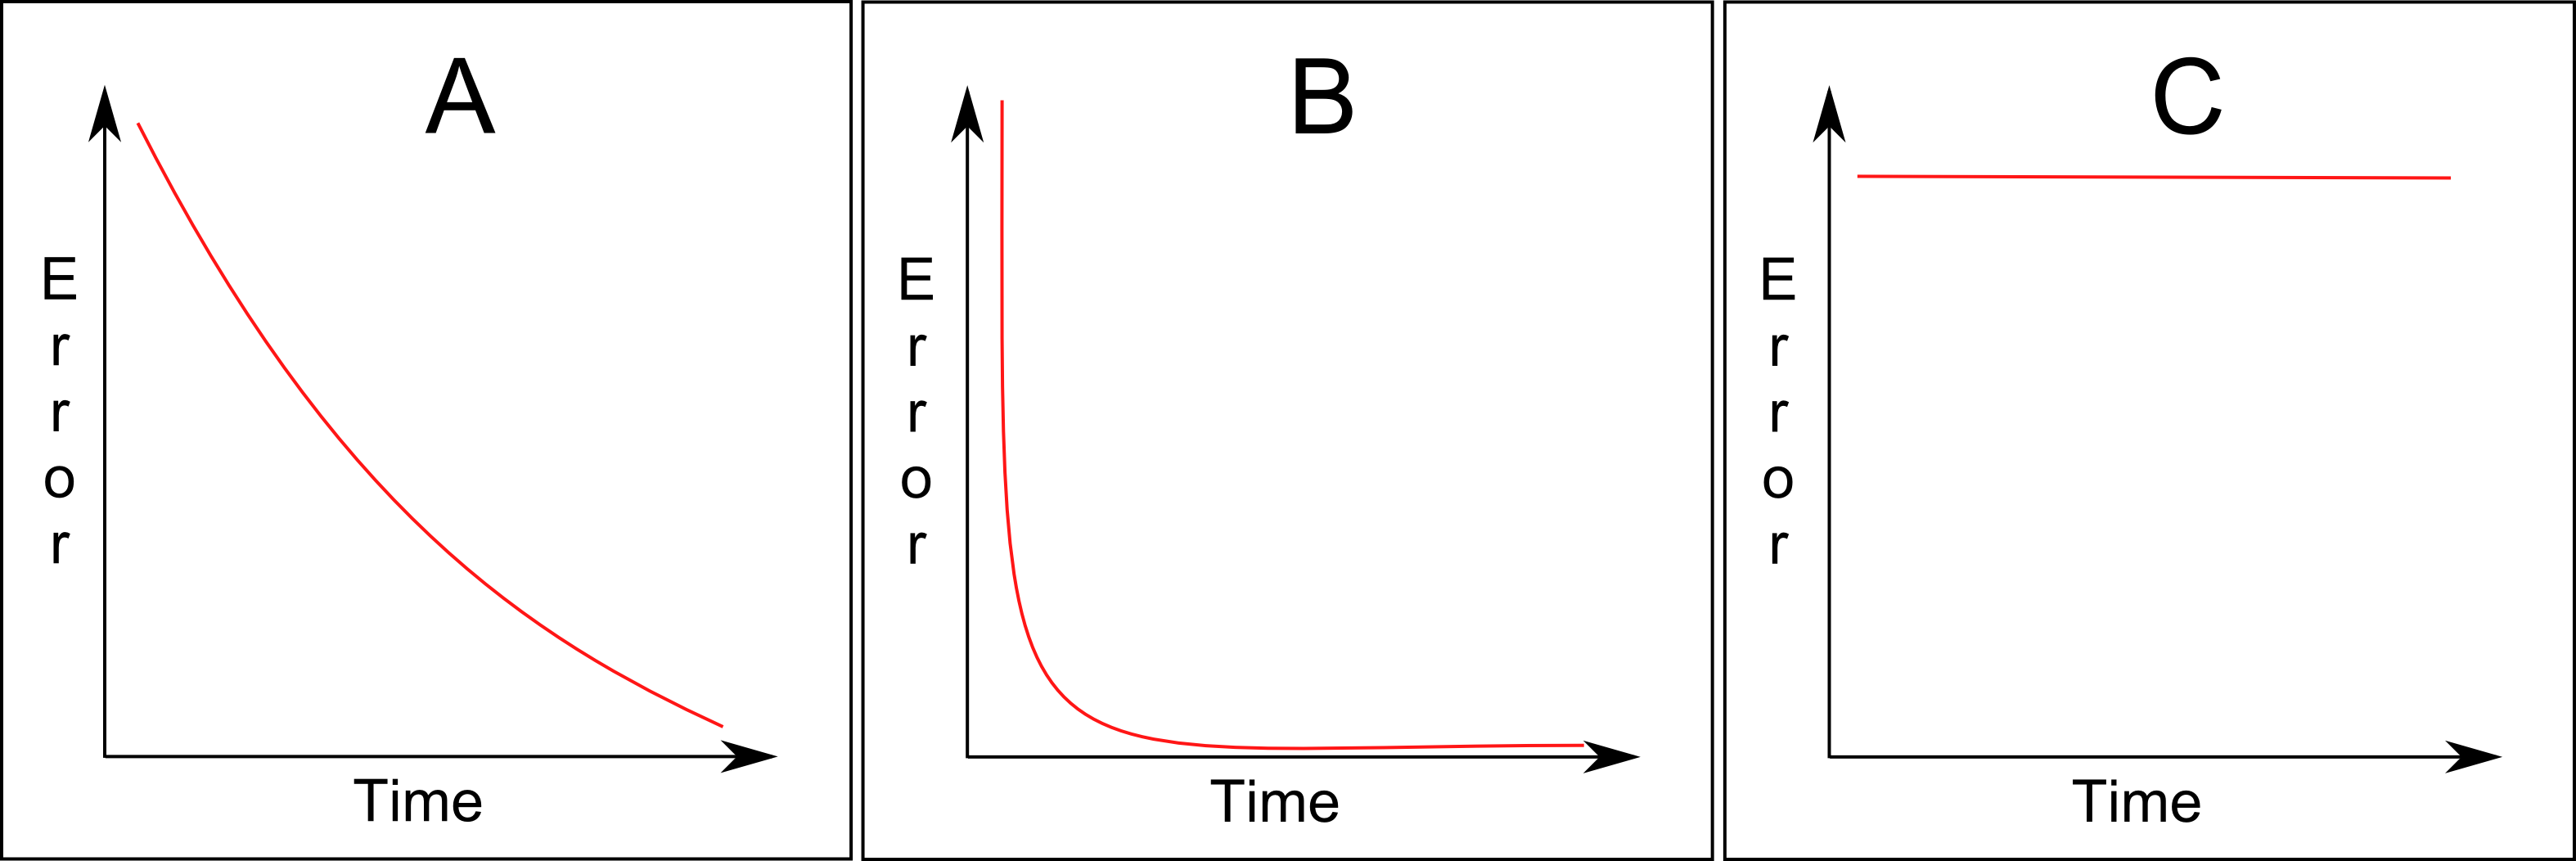
\includegraphics[scale=0.39]{img/improvement}
\caption{An interesting problem should produce a curve like graph A. A trivial problem will produce a curve like graph B, and will not score highly on the interestingness measure as the initial random fitness will likely be much higher, making the relative progress smaller. Too difficult a problem will produce a curve like graph C, and will not score highly as there will have been little to no improvement in fitness at all.}
\label{fig:graph_improvement}
\end{figure}


\begin{table}[ht]
\caption{Constant Values}
\label{tab:const}
\begin{tabular}{l | c}
\hline
Constant	& Value \\
\hline
Number of Landscape Vertices	& 100 \\
Number of Macro Actions	& 4 \\
Maximum Timesteps Per Run	& 400 \\
Maximum Function Evals	& 10000 \\
Population Size	& 50 \\
\hline
\end{tabular}
\end{table}

\begin{table}[ht]
\caption{Variable Parameters}
\label{tab:params}
\begin{tabular}{l | c}
\hline
Parameters & Default \\
\hline
Initial Solution Parameter $\sigma$	& 10 \\
Thrust Limit & 20 \\
Gravity	 & 20 \\
Velocity Loss Factor & 1.0 \\
Landscape Seed & 104353 \\
Number of Landing Pads	& 1 \\
Landing Pad Width (Vertices)	& 5	 \\
Survivable Velocity Threshold	& 15 \\
Initial Fuel	& 10000 \\
\hline	
\end{tabular}	
\end{table}

\section{Results}

\subsection{Evolving Individual Parameters}

\begin{table}[ht]
\caption{Varying Individual Parameters Alone}
\label{tab:single}
\begin{tabular}{l | c | c}
\hline
Parameter & Best Value & Best $f_{p}$ \\
\hline
Initial Solution Parameter $\sigma$	& 0.28 & 0.63 \\
Thrust Limit & 155 & 0.33 \\
Gravity	 & 3.13 & 0.50 \\
Velocity Loss Factor & 0.01 & 6 \\
Landscape Seed & 1 & 147 \\
Number of Landing Pads	& 9 & 0.37 \\
Landing Pad Width (Vertices)	& 5 & 0.37	 \\
Survivable Velocity Threshold	& 89 & 0.38  \\
Initial Fuel	& 9837 & 0.37 \\
\hline	
\end{tabular}	
\end{table}

\begin{figure}[hbtp]
\centering
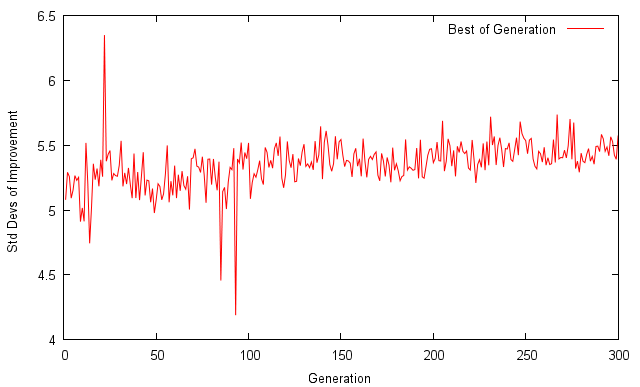
\includegraphics[scale=0.4]{img/graph_varyingvelloss}
\caption{The progress of a problem population evolving to produce interesting problems, with the only parameter varying being the velocity loss factor. Barely any improvement is made at all as a result of varying only this one parameter.}
\label{fig:graph_varyingvelloss}
\end{figure}

In initial investigation, problems were evolved with only a single dimension of change. All other parameters were set to their default values. Each of the individual parameters, as listed previously, became the individual focus of specific evolutionary runs. This was carried out to investigate which of these parameters had the most dramatic impact on the ending level of interestingness for the problem. However, more interestingly enough, it became apparent that the majority of individual parameters did not greatly impact the interestingness of the problem. One of the parameters which did have much of a noticeable effect, the velocity loss factor, did not do much to improve the interestingness of the problem over the course of an evolutionary run. 

A reason for the velocity loss factor having much of a trend and impact on the interestingness of the problem is likely related to affecting the difficulty of the problem. With the physics as defined earlier, the inertia of a ship is one of the obstacles to be challenged and overcome. However, with the velocity loss factor approaching but not equalling zero, both of the angular and linear inertia of the ship become less and less of an obstacle to overcome, as well as less present at all. Therefore, as the velocity loss factor approaches zero, the problem becomes easier, and as the problem becomes easier, the capacity for improved progress of an evolutionary run becomes greater also.

Most interestingly, parameters that do little to affect the progression of problem evolution by themselves produce values within the same range of roughly 0.3 standard deviations of improvement. Even parameters that would seem to have an impact on the progress of solutions individually do not always when only said parameters are permitted to change.

Curiously, only adjusting the landscape seed for the random generation of terrain lead to a wildly random evolutionary course of progress with no clear trends. However, given the landscape seed only affects the terrain generation, this is more useful as a measure of the highest, entirely chance based improvement that could be achieved with the default problem parameters, given a completely random landscape shape. Comparing the result of 147 standard deviations to the result of 179124 standard deviations of improvement from a later example of a problem candidate, as depicted in Table \ref{tab:example}, indicates that there could likely be considerable improvement to be made on these default parameters. This improvement existing at all, however, suggests that the physical landscape shape can completely change the progress that can be made in this type of problem.

\subsection{Evolving All Parameters}

\begin{table}[ht]
\caption{Example Evolved Parameter Set}
\label{tab:example}
\begin{tabular}{l | c}
\hline
Parameter & Value \\
\hline
Initial Solution Parameter $\sigma$	& 68.26 \\
Thrust Limit & 0.00007 \\
Gravity	 & 9.92 \\
Velocity Loss Factor & 0.34 \\
Landscape Seed & 0.00 \\
Number of Landing Pads	& 1 \\
Landing Pad Width (Vertices)	& 4	 \\
Survivable Velocity Threshold	& 1.08 \\
Initial Fuel	& 55654 \\
Proximity Weight & 1.82 \\
Velocity Weight & 7.31 \\
Fuel Weight & 5.07 \\
Angle Weight & 5.14 \\
\hline
{\bf Improvement} & {179124 $\sigma$} \\
\hline
\end{tabular}	
\end{table}

\begin{figure}[hbtp]
\centering
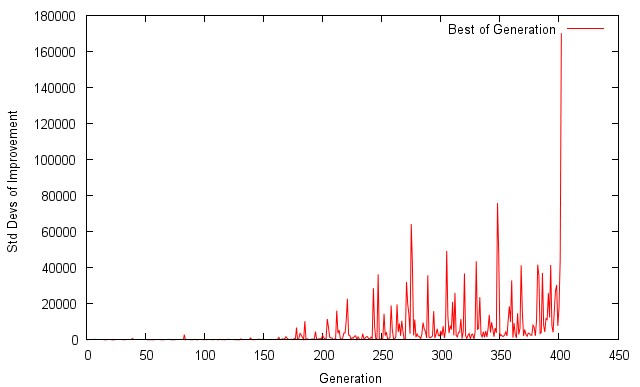
\includegraphics[scale=0.4]{img/graph_evoproblems}
\caption{The progress of a problem population evolving to produce interesting problems, with all parameters of the problem free to change. Improvement is erratic for multiple generations until a single highly effective set of parameters is found. These parameters are listed in Table \ref{tab:example}.}
\label{fig:graph_evoproblems}
\end{figure}

Interestingly, as can be seen in Figure \ref{fig:graph_evoproblems}, the course of evolution for many problems tends to be very erratic for multiple generations, with improvements being made and then discarded, until eventually a theoretically ground-breaking result is found. The exact reason for this trend is unclear at this stage, but usually coincides with a solution being found with a very low initial standard deviation for generating the initial set of solutions, or a very low thrust limit for solutions to use. However, the excessively large value that leads to this outcome indicates that there are some serious inadequacies in the measure being used. This sudden increase does not directly indicate whether the progress being made is significant, especially as the tendancy is towards producing a smaller initial standard deviation of fitness within the population.

Curiously, many of the most effective solutions have managed to meet the simple interestingness measure's implied demands either by beginning with a low initial standard deviation for generation, or by enforcing a minimal thrust limit to lead to a low initial diversity of solutions. The latter can be seen as one of the example best problem parameter sets as given in Table \ref{tab:example}. In effect, what appears to happen is the initial random population, when tested, all measure very similar. This implies a problem that cannot be solved readily through random unguided generation of solutions, but for which improved solutions are found in spite of this initial analysis. Given the highly subjective nature of what makes a problem truly interesting, it could be argued that this measure has lead to the generation of trivial problems, but it could be argued that the low initial standard deviation suggests that these problems are anything other than trivial.

When combined together, the parameters that appear to affect a problem's interestingness the most are parameters such as the velocity loss factor, the size and number of landing pads, the amount of initial fuel and the survivable velocity threshold. These factors directly impact on the difficulty of a problem. Such variances determine whether or not a problem is simpler to solve, but given that the inner problem is a problem based around minimising the error, there is a limit to how much improvement can be made when presented with an easier problem. As a result, simple or trivial problems are not rewarded as highly for problems that begin with incredibly difficult solutions that can be effectively solved through evolutionary means. The end result is a compromise, wherein the size and number of landing pads do not stray far from their original defaults, but where often more fuel is given than for the default, suggesting that the default arbitrary fuel amount was too low for practical problems within the class of problems. The velocity loss factor has already been discussed, but its impact on problems is still as apparent when it is not the only parameter being varied.

\subsection{Co-evolution of Parameters and Weights}

One of the more interesting consequences of evolving both the parameters and weights of the problem is the way the two reinforce each other to produce a better environment for solution progress. As can be seen in the example set of evolved problem parameters in Table \ref{tab:example}, the fuel weighting is much higher than the default, and the initial amount of fuel given to the ships in the inner problem is significantly higher than the default value. As can also be seen, the weighting for landing as slowly as possible under a threshold has become the highest weighted sub-condition in this example problem, and to coincide with that the thrust limit is very small, the velocity loss factor is also small to reduce inertia as much as possible, and the survivable velocity threshold has also been made very small to strongly promote ships that land within this limit. However, because this threshold is very small, it would mean a random solution has much less of a chance to solve the problem well, based on how biased the scoring is towards ships that land with a lower ending velocity. This creates a situation where the progress of evolution within this problem will be significantly higher with a guided approach than a purely random approach to solving it, which is an interesting situation to examine, as opposed to a problem where pure random chance has a good probability of solving the problem to begin with.

Another interesting example to look at lies in evolved problems that place a higher emphasis on fuel weighting. This means that quantitatively better problems in the adjacent space of possible problems require higher initial fuel, and the two parameters reinforce each other as the course of evolution continues. In cases where fuel weighting is close to zero, the fuel value does not undergo much directed change, and instead drifts randomly as other conditions become more highly weighted. This split of focus either on the fuel measure or on other measures is common across generated problem candidates, and suggests that the fuel sub-condition is in competition with the other sub-conditions. This makes sense, as the other three sub-conditions all require the expenditure of fuel to reduce the speed, adjust the position and adjust the orientation of the ship to as close to an optimal velocity, position and orientation as possible. Despite this, there exist examples where the velocity and fuel sub-conditions both have an emphasis, as in Table \ref{tab:example}. Of the sub-conditions most affected, the velocity sub-condition is usually the most directly affected, as the fuel required to slow down and approach the landing pad far exceeds that for adjusting position and orientation.

The weighting of the proximity sub-condition and the size and availability of landing pads also appear to impact each other. With a higher availability of landing pads, the proximity sub-condition becomes easier to fulfil and so leads to an improvement in the fitness of the population of solutions. As there is now an improvement in the progress of solutions, the problem itself becomes considered more interesting, and as a result problems with more and larger landing pads rewarding the proximity to a landing pad become regarded as more interesting, and dominate the population for that evolutionary run.

\section{Conclusion}

In this paper we have evolved candidates for problems within a class of related problems based upon landing a simplistic spaceship vehicle onto a jagged landscape much as in the game of {\itshape Lunar Lander}, while being mindful of one or many conditions of this landing.

These problem candidates have been evolved in accordance with a simple statistical measure of improvement. This measure is based upon multiples of the standard deviation of initial fitnesses. These initial fitnesses have been calculated from an initial random population of solutions within the environment of the problem candidate. This measure has been effective in leading to the generation of interesting problems within the space of problems relating to this {\itshape Lunar Lander} inspired case study.

The interaction and co-evolution between the problem and solution spaces examined have lead to interesting environments with unexpected changes to the physics of the problem. These environments have lead to interesting solutions that exploit these emergent characteristics of these environments. These solutions then affect the environment itself based on their performance improvement. Problems that are impossible to solve do not share this characteristic, and are discarded as less interesting than their counterparts that allow for effective solutions. In doing this, only problems that are not just solvable, but possible to get good results from have emerged from these requirements, which bring interesting new rules to a game space similar to but distinct from the original {\itshape Lunar Lander}. 

It is entirely possible that the results presented within this paper are heavily impacted by the particular choice of encoding for actions, and that a different representation may have resulted in different results. However, there are only so many possible actions within this environment, and the definition of the measure of interestingness is based on the success of solutions and not their actual content. It may be just as likely that a different encoding for actions or a different controller would produce similar results with only minor differences.

While we have examined the level of interestingness for a variety of parameter combinations within the {\itshape Lunar Lander} context, it is clear that this is a very mechanical way of determining the interestingness. As the interestingness measure ties into how well a computer controller can play the game, there are necessarily differences between how a human player might perceive the interestingness of a particular scenario and the value produced by the interestingness measure. It is perhaps safe to assume that there would be some connection, as an impossible game is not fun for a human player, and neither is a trivial game. However, the capacity for the computer controller to perform manoeuvres that a human player could not through frame-perfect course changes means it can easily be the case that a human player could struggle with a set of game parameters rated high in interestingness. Likewise, human ingenuity can be more than capable of solving some games that the software cannot. Future work comparing the reactions of human players to what the interestingness measure predicts for a given set of game parameters would be useful in determining how applicable this or similar measures could be in game design.

Ultimately, the measure used is not without some issues. The example result of a run given produces far too high a value to indicate anything very useful, especially as it is the result of manipulating conditions such that the denominator of the function used, the standard deviation of a random population's fitness, is as low as possible. While some common sense can be applied to interpreting the outcomes of these attempts to generate interesting sets of problem parameters, it is clear that this cannot apply to an entirely automated process. While there exist such flaws in this simple statistical measure of improvement, it does not appear to be without merit altogether. There exists plenty of scope for improvement upon this measure.  Further examination in different contexts and case studies would also be a useful effort. What defines a problem as ``interesting" to solve will always be a highly subjective matter, but it is considered that this attempt to define a measure of problem interestingness that is simple and fast to compute, as well as intuitive, is computationally beneficial in guiding the evolution of more interesting and solvable problems belonging to wider problem class.
 
% Use \section* for the acknowledgments
\section*{Acknowledgements}
Samuel Roberts is supported by an EPSRC PhD Studentship.


\bibliographystyle{IEEEtran}
\bibliography{difficultybib}
\end{document}
